\textit{by Alexandre Alves, Tathagata Ghosh, and Kuver Sinha}

Searches for double Higgs pair production in the $b\bar{b}\gamma\gamma$ channel are an important target for the future. In this section, we study this problem at the 14 TeV LHC in two steps, following \cite{Alves:2017ued}: 

$(i)$ We first propose a Bayesian optimization approach to select cuts on kinematic variables and study its performance compared to manual and random cuts, taking into account systematic uncertainties. We demonstrate our results with the Python algorithm \texttt{Hyperopt }.

$(ii)$ We next perform a joint optimization of kinematic cuts and boosted decision trees (BDT) hyperparameters to further discriminate signal and background events.  For our calculations, we use the \texttt{XGBoost }  implementation of BDTs for Python. 

\subsubsection{Signal and Backgrounds}

For the simulation of the signal, we use {\tt MadGraph5\_aMC@NLO\_v2.3.3}~\cite{MG5}, to generate $p p \rightarrow h h$ process exclusively at the leading order (LO). The simulation of our signal
include both the triangle and box diagrams. We scale our LO cross-section by the partial NNLO K-factor of 2.27~\cite{deFlorian:2013uza}, calculated in the large quark mass limit and use the resulting production cross section of 36.8 fb.

The following backgrounds were taken into account in our study: $(i)$ $b\bar{b}\gamma\gamma$; $(ii)$ $Zh$ with $Z \rightarrow b\bar{b}$ and $h \rightarrow \gamma\gamma$; $(iii)$ $b\bar{b}h$ with $h\to\gamma\gamma$; $(iv)$
$t\bar{t}h \rightarrow b\bar{b}+\gamma\gamma+X$; $(v)$ $jj\gamma\gamma$ where the light-jets $jj$ are mistaken for a $b$-jet pair in the detector; $(vi)$ $b\bar{b}jj$,  where the light-jets $jj$ are mistaken for a photon pair; $(vii)$ $c\bar{c}\gamma\gamma$, where a $c$-jet is mistagged as a $b$-jet; $(viii)$ $b\bar{b}\gamma j$, where one light-jet is mistaken for a photon; $(ix)$ $c\bar{c}\gamma j$ where the $c$-jets are mistagged as bottom jets and the light-jet as a photon. We note that the $b\bar{b}\gamma j$, $c\bar{c}\gamma\gamma$, and $c\bar{c}\gamma j$ backgrounds were neglected in several early studies. 
 
The cross section normalizations for the backgrounds from $(i)$ - $(v)$ are taken from ref.~\cite{Azatov:2015oxa}, which we consider reliable. In order to obtain the distributions of the kinematic variables of interest, we pass our simulated events to {\tt PYTHIA\_v6.4}~\cite{pythia} for showering, hadronization and underlying event and finally to {\tt DELPHES\_v3.3}~\cite{delphes} for detector simulation. For all further details of our signal and background simulation, we refer to our paper \cite{Alves:2017ued}. 

The following basic cuts were applied on both signal and background:
%
\begin{eqnarray}
& & p_T(j) > 20\;\hbox{GeV},\; p_T(\gamma) > 20\;\hbox{GeV},\; |\eta(j)|<2.5,\; |\eta(\gamma)|<2.5 \nonumber \\
& & 100\;\hbox{GeV} < |M_{jj}| < 150\;\hbox{GeV},\; 100\;\hbox{GeV} < |M_{\gamma\gamma}| < 150\;\hbox{GeV}\; .
\label{cuts:basicKS} 
\end{eqnarray}
%
The number of backgrounds events after imposing the basic cuts for 3 ab$^{-1}$ of integrated luminosity is shown in Table~\ref{table:nevKS}.
%
\begin{table}[!h]
\centering
\begin{tabular}{c|c|c|c|c|c|c|c|c|c}
\hline\hline
signal & $b\bar{b}\gamma\gamma$ & $c\bar{c}\gamma\gamma$ & $jj\gamma\gamma$ & $b\bar{b}\gamma j$ & $t\bar{t}h$ & $c\bar{c}\gamma j$ &  $b\bar{b} h$ & $Zh$ & total backgrounds \\ 
\hline
42.6   & 1594.5  & 447.7   &  160.3 &   137 & 101.1  & 38.2  &  2.4    & 1.8 & 2483 \\
\hline\hline
\end{tabular}
\caption{The number of signal and the various types of backgrounds considered in this work after imposing the basic cuts of eq.~(\ref{cuts:basicKS}) for 3 ab$^{-1}$ of data. We found $b\bar{b} jj$ negligible after cuts and after estimating the probability of the jet pair faking a photon pair.}
\label{table:nevKS}
\end{table}

\subsubsection{Bayesian Optimization}

The $b\bar{b}\gamma\gamma$ channel has been studied by several groups using cut and count strategies. Once signal and background cross sections are normalized to the proper values, one finds that the analysis of any particular group does not radically outperform that of any other. For a detailed comparison, we refer to Table 2 of \cite{Alves:2017ued}. 

Bayesian optimization  offers a systematic way to obtain the most optimal cuts on a set of kinematic variables. The algorithm we utilize is implemented in the Python library \texttt{HyperOpt}~, based on the so-called sequential model-based optimization (SMBO) technique \cite{Bergstra1, Bergstra2, url:hyperopt}. 
%This class of algorithms suggests a new model (a new configuration of parameters) at each iteration in order to optimize the criterion of Expected Improvement (EI), which is the expectation that under a model $M$ of a function $f$, $y=f(x)$ will exceed some threshold $y^c$
%\begin{equation}
%EI_{y^c}(x)=\int_{-\infty}^{+\infty} \max(y^c-y,0)p_M(y|x)dy
%\end{equation} 
%in the search for the minimum of $f$. 
%The maximum search is just a matter of looking for the minimum of $-f$.

%The major challenge in computing $EI(x)$ is estimating the conditional probability $p_M(y|x)$. \texttt{HyperOpt} overcomes this difficulty by means of the Bayes rule, $p_M(y|x)=\frac{p(x|y)p(y)}{p(x)}$, where $p(x)$ is an assumed prior distribution of the parameters. By keeping a sorted list of observations of $y=f(x)$, it is possible to compute the quantiles $\gamma=p(y<y^c)$, while $p(x|y)$ is a non-parametric distribution estimated from previous observations along the run of the algorithm. The strategy to evaluate $p(x|y)$ in \texttt{HyperOpt} is known as a Tree-structured Parzen Estimator approach, TPE for short. In TPE, $p(x|y)$ equals $\ell(x)$($g(x)$) if $y<y^c$($y\geq y^c$), thus providing a non-parametric estimate of $p(x|y)$ from previous runs of the algorithm. 

%\begin{figure}[!t]
%\centering
%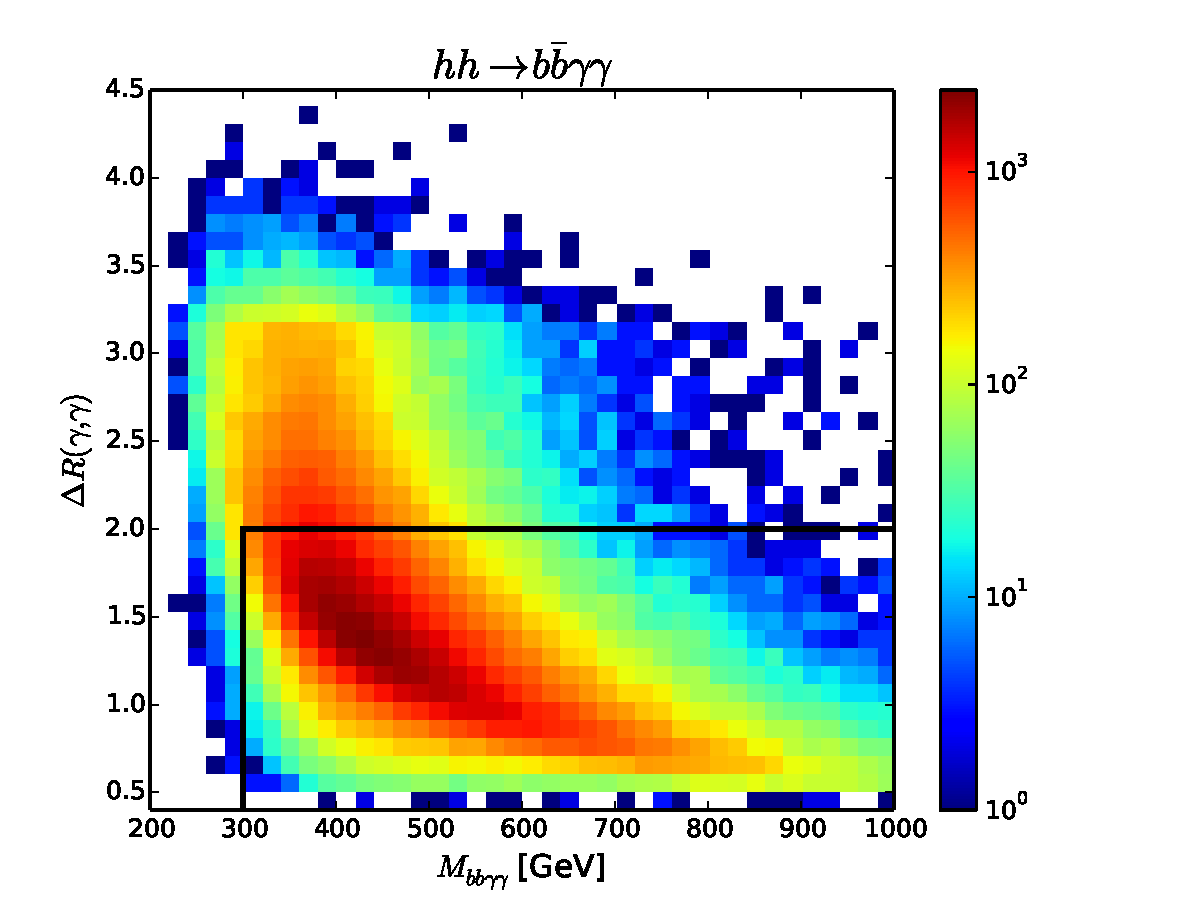
\includegraphics[scale=0.35]{correlation_signal_HHH.pdf}
%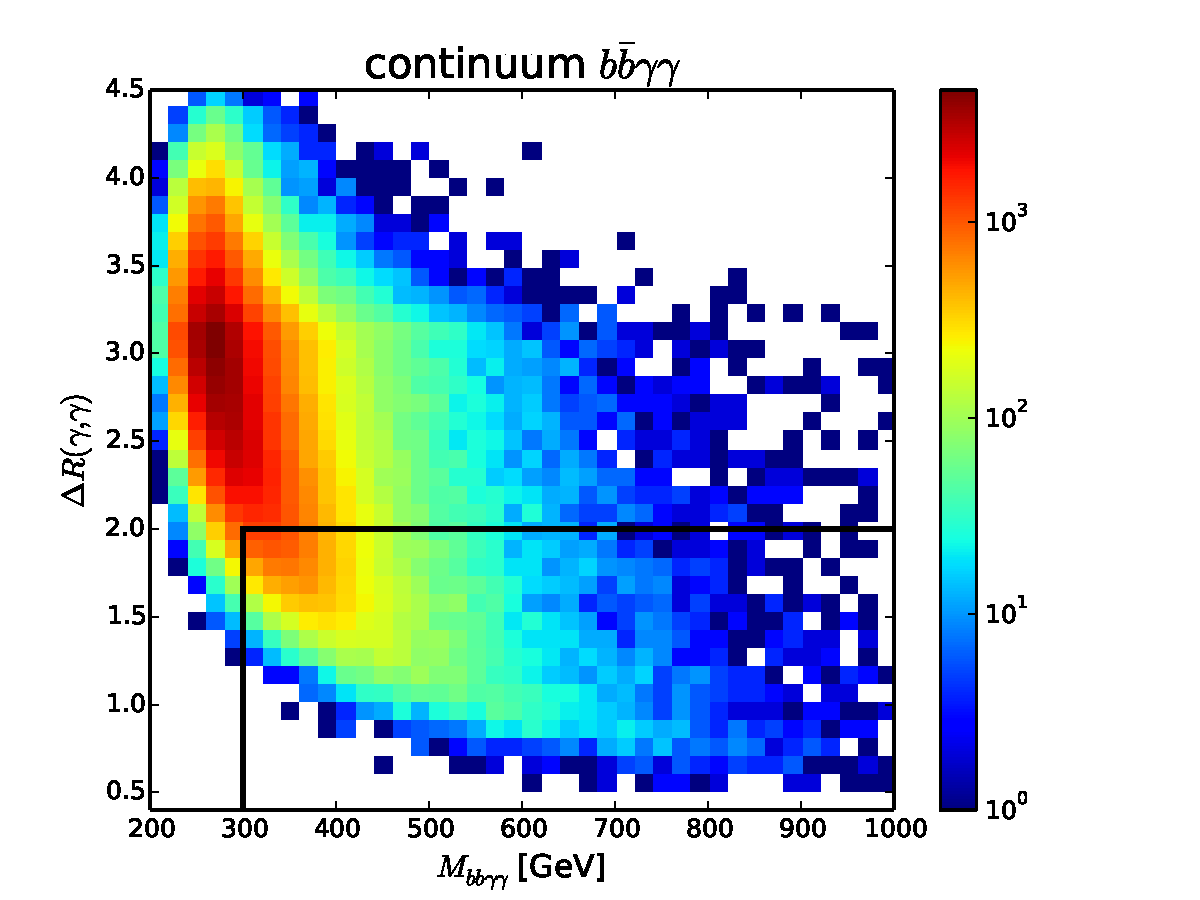
\includegraphics[scale=0.35]{correlation_back_HHH.pdf}
%\caption{\textbf{Left panel:} The invariant mass of two $b$-jets and two photons. Kinematic distributions of the signal (shaded red), and the backgrounds $b\bar{b}\gamma\gamma$ (black), $t\bar{t}h$ (blue) and $Zh$ (green) are displayed.  \textbf{Right panel:} In (b), we show the transverse momentum of a pair of photons. 
%}
%\label{fig:4}
%\end{figure}
%


The  kinematic variables used in our  study are:
$(i)$ transverse momentum of $b$-jets and photons: $p_T(b)$ and $p_T(\gamma)$; 
$(ii)$ $b\bar{b}$ and $\gamma\gamma$ invariant masses: $M_{bb}$ and $M_{\gamma\gamma}$, where signal events exhibit resonance peaks at $m_h$;
$(iii)$ transverse momentum of $b\bar{b}$ and $\gamma\gamma$: $p_T(bb)$ and $p_T(\gamma\gamma)$; 
$(iv)$ invariant mass of two $b$-jets and two photons: $M_{bb\gamma\gamma}$;
$(v)$ distance between pairs of $b$-jets and photons: $\Delta R(bb)$, $\Delta R(\gamma\gamma)$ and $\Delta R(b\gamma)$, where
$\Delta R=\sqrt{(\Delta\eta)^2+(\Delta\phi)^2}$ in the pseudo-rapidity and azimuthal angle plane $(\eta,\phi)$;
$(vi)$ the fraction $E_T/M_{\gamma\gamma}$ for the two hardest photons in the event; these are variables used in experimental searches as in ref.~\cite{Aad:2014yja, CMS}.

In Figure~\ref{fig:BayesianKS}, we display the results obtained from the Bayesian optimization of cuts on the above kinematic variables. We see that after 100-200 trials, the signal significance does not change much and the optimized cuts achieved a significance of 2.81$\sigma$ against 2.1$\sigma$ of the manual search of ref.~\cite{Azatov:2015oxa}, a 34\% improvement. If $b\bar{b}\gamma j$, $c\bar{c}\gamma\gamma$, and $c\bar{c}\gamma j$ backgrounds are incorporated, the Bayesian search reached 2.48$\sigma$ against 1.85$\sigma$ of the cuts of ref.~\cite{Azatov:2015oxa}, again roughly the same improvement. %A larger $S/B$ was also achieved as shown in table~\ref{table:3}. 
The performance of the Bayesian algorithm is also displayed in Figure~\ref{fig:BayesianKS}.

\begin{figure}[!t]
\centering
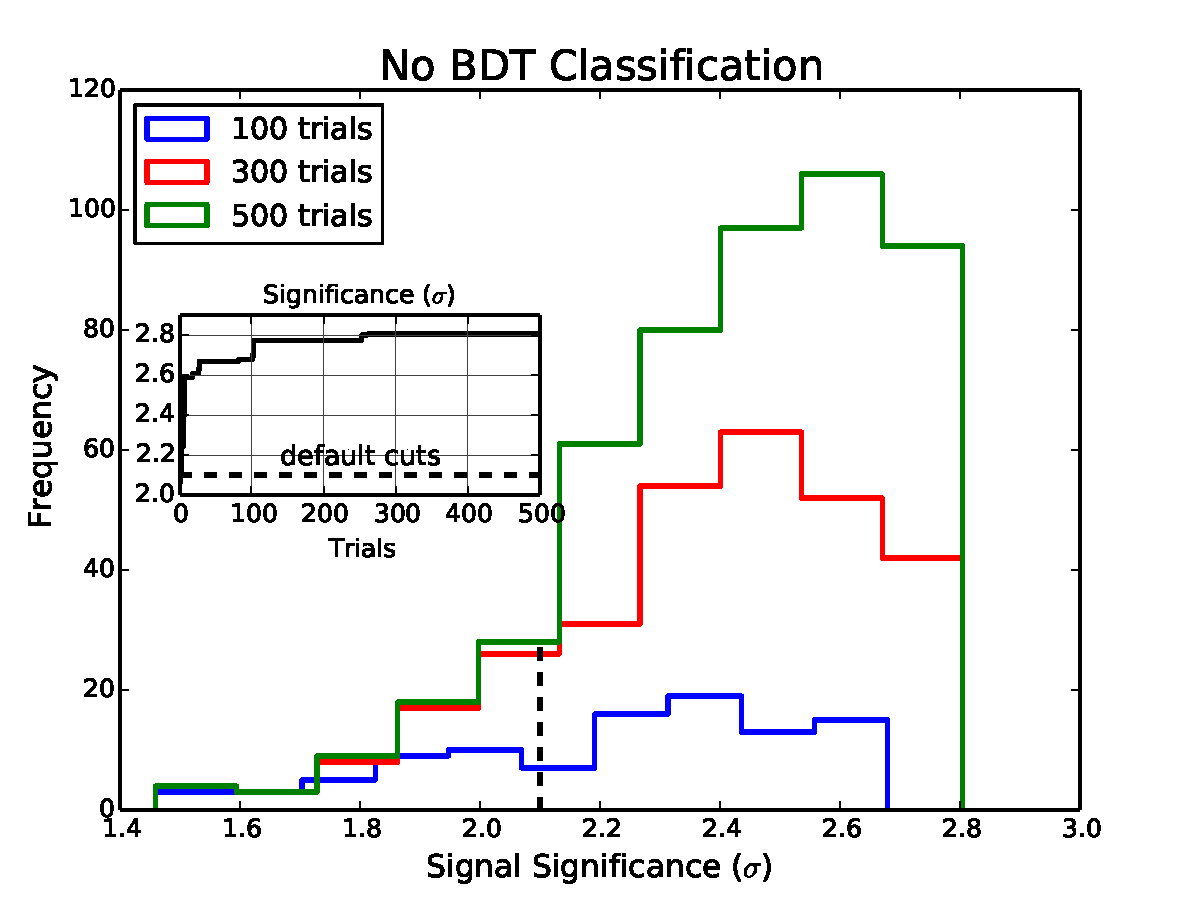
\includegraphics[scale=0.35]{./section3/plots/improve_HHH_cuts.pdf}
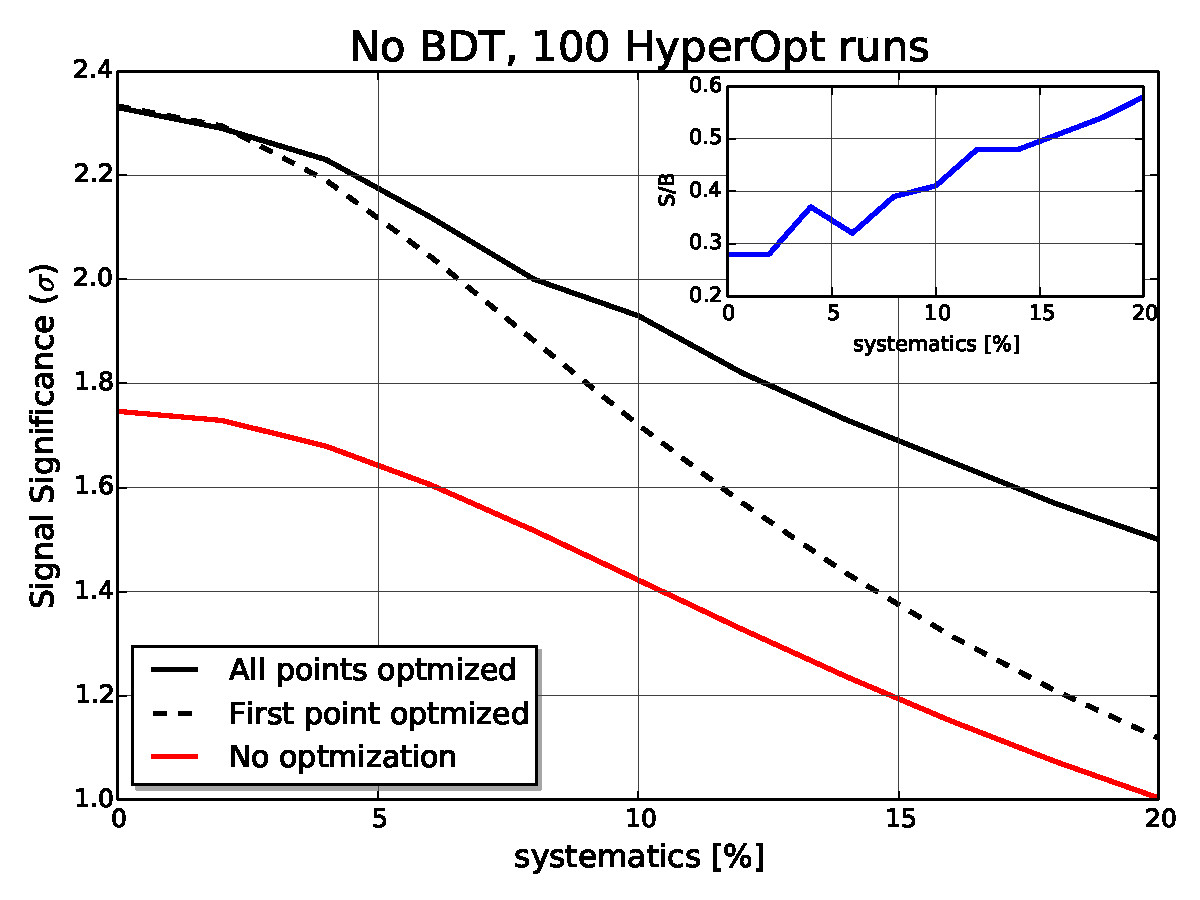
\includegraphics[scale=0.35]{./section3/plots/ams_HHH_sys_compare.pdf}
\caption{\textbf{Left panel:} The left panel shows the optimized search with the TPE algorithm in \texttt{HyperOpt} with no systematic errors. The inset frame in the left plot shows the significance as a function of the number of trials. $S/\sqrt{B}$ is used to compute the signal significance. The black dashed line represents the results obtained with the cuts of Azatov \emph{et. al.}, ref.~\cite{Azatov:2015oxa}. \textbf{Right panel:} The $S/\sqrt{B+(\varepsilon_B B)^2}$ significance metric as a  function of $\varepsilon_B$, the systematic uncertainty in the total background rate. The red line represents the default cuts of Azatov \emph{et. al.}, the black dashed assumes an optimized strategy just for the 0\% systematics point, while for the solid upper line, the algorithm was solicited to learn the best cuts for each systematics level from 0 to 20\%. In the inner plot we show the $S/B$ ratio for the point-to-point optimization case. }
\label{fig:BayesianKS}
\end{figure}
%


\subsubsection{BDT Analysis}

We now turn to a discussion of the BDT analysis, for which we utilize the \texttt{XGBoost}  implementation of BDTs for Python. \texttt{XGBoost} is chosen for its good discrimination performance, speed and capacity of parallelization.  For our  analysis we simulated $\sim 880000$; depending on the cuts, however, the total number of events usually drops to around $100000$--$300000$ events which also turned out to be a sufficient number of samples to keep overfitting under control.

Using \texttt{HyperOpt}, we perform a joint optimization of the kinematic variables introduced previously in conjunction with the following BDT hyperparameters: the \texttt{number of boosted trees}, the \texttt{learning rate}, the \texttt{maximum depth of the trees}, and the minimum sum of instance weight needed in a child to continue the splitting process of the tress, \texttt{min\_child\_weight}. All the BDT results were obtained from a 5-fold cross validation by randomly splitting training and testing samples at the proportion of 2/3 and 1/3 of the total sample, respectively. We allowed for 300 trials in \texttt{HyperOpt}. 

Hyperparameters like the \texttt{number of boosted trees}, \texttt{maximum depth of the trees} and the \texttt{min\_child\_weight} are directly related to the complexity of the algorithm by controlling the number, size and configuration of the trees. The \texttt{learning rate}, also known as \texttt{shrinkage} in this context, is a parameter that controls the weight new trees have to further model the data. A large value permits a larger effect from new added trees and might lead to more severe overfitting. There are other parameters which can be eventually used to prevent overfitting and loss of generalization power, but we found that tuning these parameters was sufficient to achieve a good performance.


A comparative result of a simple cut and count analysis and a sequential optimization of cuts and BDT hyperparameters are presented  Table~\ref{table:resultsbdtKS}. We note that BDT outperforms simple cut and count, even when cutting is performed using Bayesian optimization. This is due to the better discrimination between the signal and background classes achieved by the machine learning algorithms as they find more profound correlations among the kinematic features and those classes. These correlations cannot be fully explored in simple/manual rectangular cut-and-count analyses. 

%
\begin{table}[h]
\centering
\begin{tabular}{c|c|c}
\hline
systematics (\%) & Cut-and-count & BDT \\
\hline\hline 
0 & 2.34[1.76] & 3.88 \\
\hline
10 & {\bf 1.93}[1.43] & {\bf 3.57}  \\
\hline
20 & 1.51[1.0] & 3.10  \\
\hline\hline
\end{tabular}
\caption{Signal significances for cut-and-count and BDT for 0, 10 and 20\% systematics. We took all backgrounds into account for the computation of the AMS with optimized cuts and an integrated luminosity of 3 ab$^{-1}$ at the 14 TeV LHC. The bold-face numbers represent the significances expected with the level of systematics anticipated by the experimental collaborations in refs.~\cite{ATLAS14, ATLAS17, CMS}. The numbers inside brackets are the significances computed with the default cuts of Azatov \emph{et. al.}, ref.~\cite{Azatov:2015oxa}, which we took as baseline results.}
\label{table:resultsbdtKS}
\end{table}
%
%
\begin{figure}[!t]
\centering
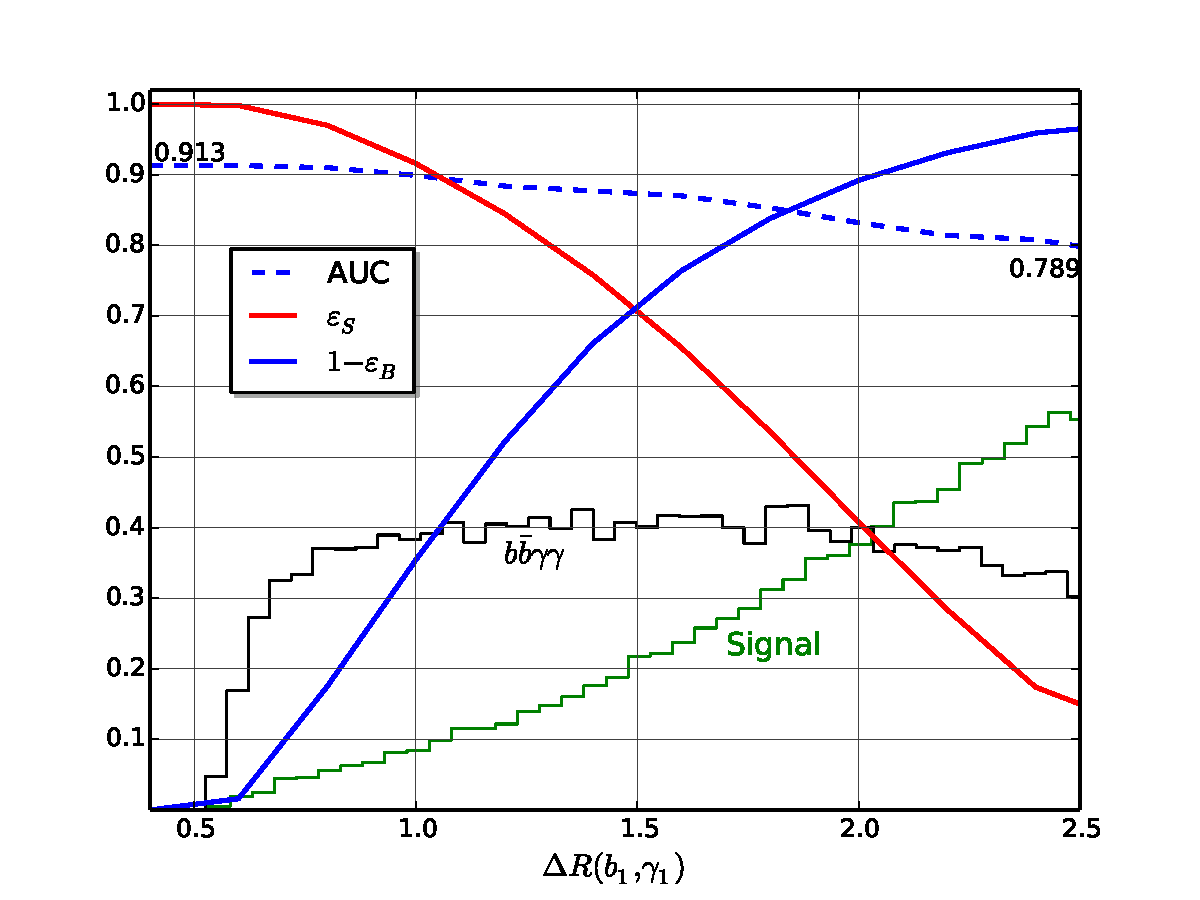
\includegraphics[scale=0.35]{./section3/plots/tradeoff_HHH.pdf}
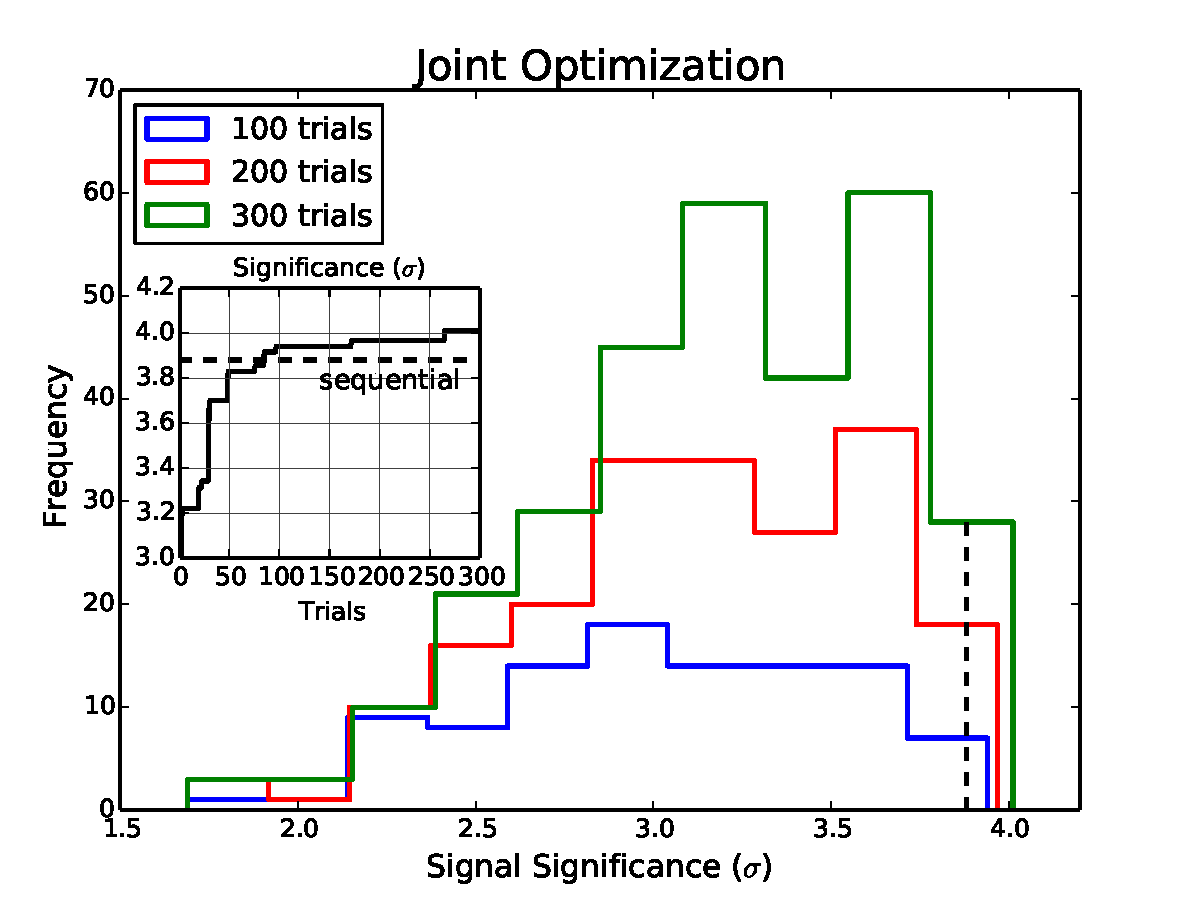
\includegraphics[scale=0.35]{./section3/plots/improve_HHH_joint.pdf}
\caption{\textbf{Left panel:}  We show the results of the effects of imposing hard cuts on $\Delta R_{b_1\gamma_1}$ for the BDT performance, see~\cite{Alves:2017ued} for further details. \textbf{Right panel:} The histogram of number of cut strategies producing a given significance interval in a BDT-aided classification analysis. The inset plot shows the significance as a function of the number of \texttt{HyperOpt} trials. No systematics are assumed, the backgrounds are those of ref.~\cite{Azatov:2015oxa} and the $S/\sqrt{B}$ used to compute the signal significances. The black dashed line represents the results obtained with the default cuts of Azatov \emph{et. al.}, ref.~\cite{Azatov:2015oxa}.}
\label{fig:8resultsKS}
\end{figure}
%
However, there is a trade-off between the efficiency of the cuts and the ML performance which is usually neglected in phenomenological works where these tools are employed. The reasoning is simple: cutting harder cleans up more backgrounds but weakens the correlations between the kinematic variables and the event classes, thereby decreasing the ML performance. On the other hand, relaxing the cuts makes the correlations stronger helping to boost ML but the discrimination power gained might not be enough to get a good significance with a large number of surviving back- ground events. Hence, a joint optimization of cuts and BDT hyperparameters improve the performance of our analysis further. 
%Finding the optimal performance from this competition is the core of the method present in the section. In short, a joint optimization of cuts and BDT hyperparameters improve the performance of our analysis further.  
 


The maximum AMS significance is 4.0$\sigma$ for a joint optimization analysis of cuts and BDT hyperparameters. The final selections of the kinematic variables and BDT hyperparameters are the following $ p_T(1) >72\; \hbox{GeV},\; p_T(2) >20\; \hbox{GeV}; \Delta R_{ij}>0.15,\; \Delta R_{ii}<3.6; M_{b\bar{b}\gamma\gamma}>370\; \hbox{GeV},\; p_{T_{ii}}>145\; \hbox{GeV},\; M_{b_1\gamma_1}>100\; \hbox{GeV}; |M_{bb}-m_h|<27\; \hbox{GeV},\; |M_{\gamma\gamma}-m_h|<11\; \hbox{GeV}; \hbox{\texttt{number of trees}}=157; \hbox{\texttt{learning rate}}=0.101; \hbox{\texttt{maximum tree depth}}=14; \hbox{\texttt{min\_child\_weight}}=5$. We have denoted $p_T(1)$ as the leading $b$-jet or photon, and $p_T(2)$ as the next-to-leading $b$-jet or photon.

The results are shown in Figure~\ref{fig:8resultsKS}. The left panel 
shows the normalized $\Delta R_{b_1\gamma_1}$ histograms for the signal and the $b\bar{b} \gamma \gamma$ continuum background, the signal efficiency (background rejection) is the red (blue) line, and the area under the Receiver-Operator curve (ROC), AUC, is the dashed line. The bigger the AUC, the better the performance of a cut-and-count analysis based on that distribution. 
%we show the output scores of the BDT for signal and background after joint optimization of kinematic variables and hyperparameters using \texttt{HyperOpt}. 
On the right panel, we show the histogram of number of cut strategies producing a given significance interval in a BDT-aided joint optimization analysis. Finding this optimal performance from the competition between hard cuts and an ML algorithm is the core of the method presented in the section.